
%----------------------------------------------------------------------------------------
%	Lecture 6
%----------------------------------------------------------------------------------------

\chapter{Exponentials and Log, Logarithmic Differentiation, Hyperbolic Functions}

\bigbreak
\section{Taking derivatives of expinentials and logarithms}

\subsection{Today's main task : find $\diff{}{x} a^x$}

We can write $$ \diff{}{x} a^x = \lim_{\Delta x \to 0} \frac{a^{x+\Delta x} - a^x}{\Delta x} $$

We can factor out $a^x$ : 
$$ \lim_{\Delta x \to 0} \frac{a^{x+\Delta x}-a^x}{\Delta x} 
	= \lim_{\Delta x \to 0} a^x \frac{a^{\Delta x} - a^0}{\Delta x}
	= a^x \lim_{\Delta x \to 0} \frac{a^{\Delta x} - 1}{\Delta x}
$$

Let's call $$ M(a) = \lim_{\Delta x \to 0} \frac{a^{\Delta x} - 1}{\Delta x} $$

We don't know what $M(a)$ is, but we can say : $$ \diff{}{x} a^x = M(a) a^x $$

Here are two ways to describe $M(a)$:
\begin{enumerate}
	\item Analytically $M(a) = \diff{}{x} a^x$ at $x=0$. \\
	Indeed, $ M(a) = \lim_{\Delta x \to 0} \frac{a^{\Delta x} - 1}{\Delta x} = \diff{}{x} a^x \big|_{x=0} $
	\item Geometrically, $M(a)$ is the slope of $a^x$ at $x=0$. 

	\begin{figure}[ht!]
		\centering        
		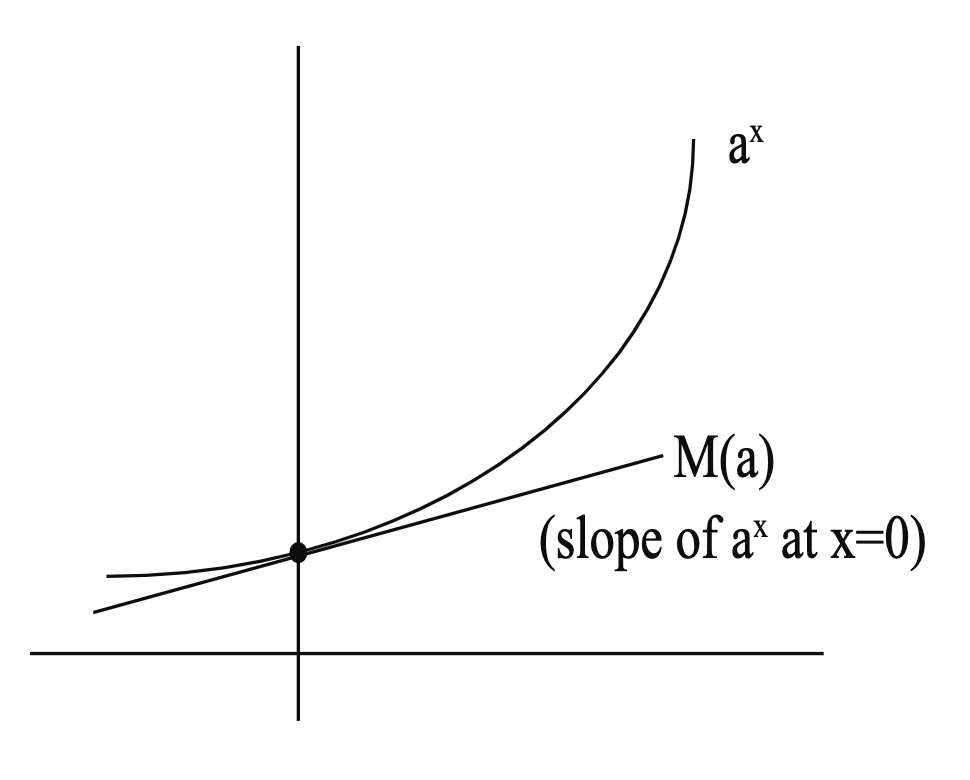
\includegraphics[scale=0.4]{./images/lecture_6_figure_1.png}
		\caption{Geometric Definition of $M(a)$}
	\end{figure}
\end{enumerate}

The trick to finding out what $M(a)$ is is to beg the question and \underline{define} $e$ as the number such that $M(e) = 1$.
Now can we be sure that there is such a number $e$?
First notice that as the base $a$ increases, the graph gets steeper continuosly and $M(1) = 0$ as $1^x = 1$ which is a constant.
So it must pass a point where $M(a) = 1$.

Thus, we \textit{define} $e$ to be the unique number such that $$ M(e) = 1 $$
or, to put it another way, $$ \lim_{h \to 0} \frac{e^h - 1}{h} = 1 $$
or, to put it still another way, $$\diff{}{x} (e^x) = 1 \text{ at } x = 0 $$
So finally, $$\boxed{\diff{}{x}(e^x) = e^x}$$


\subsubsection{Natural log (inverse of $e^x$)}

$$
\boxed{\text{If } y = e^x, \text{ then } \ln(y) = x} 
$$

Note that $e^x$ is always positive even if $x$ is negative.

Let us use implicit differentiation to find $\diff{}{x} \ln(x)$. Let $w = \ln(x)$. We want to find $\diff{w}{x}$.
\begin{equation*}
\begin{split}
	e^w & = x \\
	\diff{}{x} e^w & = \diff{x}{x} \\
	e^w \diff{w}{x} & = 1 \\
	\diff{w}{x} & = \frac{1}{e^w} = \frac{1}{x} \\
\end{split}
\end{equation*}

$$
\boxed{\diff{}{x} \ln(x) = \frac{1}{x}} 
$$

